\documentclass[12pt]{article}
\usepackage{geometry}
\geometry{
	left=20mm,
	top=20mm,
}
\usepackage[utf8]{inputenc}
\usepackage[shortlabels]{enumitem}
\usepackage{array}
\newcolumntype{C}[1]{>{\centering\let\newline\\\arraybackslash\hspace{0pt}}m{#1}}
\usepackage[spanish,es-nodecimaldot]{babel}
 \usepackage{url}
\usepackage[spanish, fixlanguage]{babelbib}
\bibliographystyle{IEEEtran}
\usepackage{graphicx}
\graphicspath{ {./images/} }
\usepackage{amssymb}
\usepackage{amsmath}
\usepackage{subcaption}
\usepackage[linesnumbered]{algorithm2e}
\newcommand\mycommfont[1]{\footnotesize\ttfamily\textcolor{blue}{#1}}
\SetCommentSty{mycommfont}
\usepackage{tikz}
\usetikzlibrary{positioning, fit}
\usetikzlibrary{babel}
\usepackage{titlesec}
\titlespacing*{\section}
{0pt}{5.5ex plus 1ex minus .2ex}{.3ex plus .1ex}
\titlespacing*{\subsection}
{0pt}{5.5ex plus 1ex minus .2ex}{2.3ex plus .1ex}
\title{Tarea 2: Clasificador bayesiano ingenuo}

\author{
	Saul Ivan Rivas Vega \\
	\\
	Aprendizaje Automatizado\\
}

\date{\today}

\begin{document}
	\maketitle
	\pagebreak
	\section{Géneros}
	  \paragraph{} Un programa de salud gubernamental desea clasificar los registros de las personas en géneros femenino (F) o masculino (M) a partir de los atributos nombre, estatura y peso. Se cuentan con los
	  siguientes registros:\\
	  \begin{figure}[h!]
	  	\centering
	  	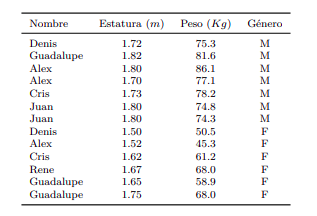
\includegraphics[width=.6\linewidth]{excercise1}
	  	\label{fig1}
	  \end{figure}
  \paragraph{} Entrena un clasificador bayesiano ingenuo usando estimación por máxima verosimilitud y otro usando estimación por máximo a posteriori. Reporta los parámetros que obtuviste en ambos casos y usa los clasificadores entrenados para predecir la clase de los siguientes vectores: x1 = (Rene, 1.68, 65), x2 = (Guadalupe, 1.75, 80), x3 = (Denis, 1.80, 79), x4 = (Alex, 190, 85) y x5 = (Cris, 165, 70).
  Describe de forma detallada el procedimiento que seguiste tanto en el entrenamiento como en la predicción y discute los resultados obtenidos.
  Para el entrenamiento del clasificador por máximo a posteriori considera los siguientes valores
  para las distribuciones correspondientes:
	  \begin{figure}[h!]
	  	\centering
	  	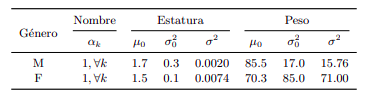
\includegraphics[width=.6\linewidth]{ex1_002}
	  	\label{fig2}
	  \end{figure}
 \subsection{Estimador por máxima verosimilitud}
 \paragraph{} Los atributos son: \textbf{nombre}, \textbf{estatura} y \textbf{peso}, y la clase es \textbf{género}.\\
 \subsubsection{Atributo \textit{Nombre}}
 \paragraph{} Para el \textbf{nombre} podemos asumir una distribución categórica:
  \begin{equation}
  \begin{split}
  X_{nombre}^{(i)}\sim Cat(X_{nombre}^{(i)};q)\\
  \end{split}
  \end{equation}
  Donde las categorías son los nombres y los podemos enumerar:
  \begin{enumerate}
  	\item Denis
  	\item Guadalupe
  	\item Alex
  	\item Cris
  	\item Juan
  	\item Rene
  \end{enumerate}
  Y así con los nombres de 1 a 6 podemos definir a $Cat(X_{nombre}^{(i)};q)$ como:\\
  \begin{equation}
  \begin{split}
  Cat(X_{nombre}^{(i)};q) = \prod_{k=1}^{6}q_{k}^{[x_{nombre}^{(i)}=k ]}\\
  \end{split}
  \end{equation}
  Donde podemos estimar a $q_k$ usando el estimador de máxima verosimilitud como:
  \begin{equation}
  \begin{split}
  \hat{q}_k =& \frac{c_k}{n} \\ 
  \text{Donde $c_k$:}&\\
  c_k =& \sum_{i = 1}^{n}{[x^{(i)}_{nombre}=k]}
  \end{split}
  \end{equation}
  Así podemos estimar el parámetro para las primer categoría:\\
  \begin{equation}
  \begin{split}
  c_1 &= \sum_{i = 1}^{13}{[x^{(i)}_{nombre}=1]}\\
  	&= 1 + 0 + 0 + 0 + 0 + 0 + 0 + 0 + 1 + 0 + 0 + 0 + 0 + 0\\
  	&= 2\\
  \hat{q}_1 =& \frac{2}{13} \\ 
  \end{split}
  \end{equation}
  Y de la misma forma para las categorías restantes:
  \begin{equation}
  \begin{split}
  c_2 = 3, \; \; \; \hat{q}_2 = \frac{3}{13} \; \; \; \; \; \; \; \; \; \; \; \; &  c_3 = 3, \; \; \; \hat{q}_3 = \frac{3}{13}\\
  c_4 = 2, \; \; \; \hat{q}_4 = \frac{2}{13} \; \; \; \; \; \; \; \; \; \; \; \; &  c_5 = 2, \; \; \; \hat{q}_5 = \frac{2}{13}\\ 
  c_6 = 1, \; \; \; \hat{q}_6 = \frac{1}{13}
  \end{split}
  \end{equation}
  \subsubsection{Atributo Estatura}
  \paragraph{}Para la \textbf{estatura} podemos asumir una distribución normal:
  \begin{equation}
  \begin{split}
  X_{estatura}^{(i)}\sim \mathcal{N}(X_{estatura}^{(i)};\mu;\sigma^2)\\
  \end{split}
  \end{equation}
  Donde $\mathcal{N}(X_{estatura}^{(i)};\mu;\sigma^2)$ se define como:\\
  \begin{equation}
  \begin{split}
  \mathcal{N}(X_{estatura}^{(i)};\mu;\sigma^2) =& \frac{1}{\sqrt{2\pi\sigma^2}}e^{\frac{-(x^{(i)} - \mu)^2}{2\sigma^2}}\\
  \end{split}
  \end{equation}
 \section{Spam}
	 
\end{document}  